% Created 2022-07-01 vr 19:23
% Intended LaTeX compiler: pdflatex
\documentclass[11pt]{article}
\usepackage[utf8]{inputenc}
\usepackage[T1]{fontenc}
\usepackage{graphicx}
\usepackage{grffile}
\usepackage{longtable}
\usepackage{wrapfig}
\usepackage{rotating}
\usepackage[normalem]{ulem}
\usepackage{amsmath}
\usepackage{textcomp}
\usepackage{amssymb}
\usepackage{capt-of}
\usepackage{hyperref}
\author{Massimiliano Falzari (s3459101)}
\date{\today}
\title{Uncertainty in Machine Learning $\backslash$\ Assignment 3}
\hypersetup{
 pdfauthor={Massimiliano Falzari (s3459101)},
 pdftitle={Uncertainty in Machine Learning $\backslash$\ Assignment 3},
 pdfkeywords={},
 pdfsubject={},
 pdfcreator={Emacs 26.3 (Org mode 9.1.9)},
 pdflang={English}}
\begin{document}

\maketitle
\tableofcontents


\section{Out of Distribution Detection}
\label{sec:orgbbd923c}

I have used an ensemble (10 NN) for epistemic uncertainty quantification and
the machine learning model is a standard Convolutional NN

The result can be seen in the table \ref{tab:org9d93816}.
The model that has the best performance is the ensemble
model. However, the difference is not too evident.

From the results, we can observe that the AUC is higher in the
ensemble than in the baseline model. The accuracies are almost identical
both for ID and OD.
In \ref{fig:org62b3204} and \ref{fig:orgdeb9a27} we can see that the
Baseline model has a higher peak around 0 for in distribution data.
This is because this model does not use any Uncertainty quantification
method and therefore is more confident resulting in lower entropy.
For out-of-distribution data, there is no clear difference in entropy between the
two models. The same is true for the max probability graphs
(\ref{fig:org270c432},\ref{fig:org9621000}), there is no clear difference
between the two models.
The ROC curves (\ref{fig:org9599962},\ref{fig:org3cd6800}) are also quite similar,
however, from the AUC value in \ref{tab:org9d93816} we can see that the ensemble method
is slightly better than the baseline model.

\begin{table}[htbp]
\caption{\label{tab:org9d93816}
Results for Out of Distribution Detection}
\centering
\begin{tabular}{lllrrr}
\hline
model & ID & OD & ID accuracy & OD accuracy & AUC\\
\hline
ensemble & mnist & fashion\(_{\text{mnist}}\) & 0.9044 & 0.1145 & 0.853628295\\
\hline
baseline & mnist & fashion\(_{\text{mnist}}\) & 0.9025 & 0.1027 & 0.846553755\\
\hline
\end{tabular}
\end{table}


\section{Reverse OOD Detection}
\label{sec:org44db352}

No, we do not obtain the same performance according to AUC. This is
because of different reasons. First, the training process is stochastic
so we should not expect the same results. Second, the features in the
two datasets are different and therefore, in general, it is not the
case that reversing the dataset in an OOD framework results in similar results.

In \ref{fig:org38b1854} we can see a quite different pattern both for in
and out distribution data with respect to \ref{fig:org62b3204}.
This is probably because Fashion mnist has more features/ more
information and therefore it is harder to learn compared to the
standard mnist dataset. Indeed, we can see that the entropy is
considerably higher both for in and out distribution data, which means
less confidence.
Similar pattern can be seen in \ref{fig:orgb9eb82d}. For in-distribution
data the model is not really confident. For out-of-distribution data,
the distribution has a really high peak of 0.2 which is completely
different in \ref{fig:org270c432}.
This again shows that Fashion mnist is harder to learn or it needs
different architecture/hyperparameters.


\begin{table}[htbp]
\caption{\label{tab:orgb97d2ed}
Results for Reverse Out of Distribution Detection}
\centering
\begin{tabular}{lllrrr}
\hline
model & ID & OD & ID accuracy & OD accuracy & AUC\\
\hline
ensemble & fashion\(_{\text{mnist}}\) & mnist & 0.7565 & 0.0715 & 0.827956175\\
\hline
baseline & fashion\(_{\text{mnist}}\) & mnist & 0.7471 & 0.0575 & 0.821769015\\
\hline
\end{tabular}
\end{table}

\section{Calibration}
\label{sec:orgf433c58}

The calibration errors are all really close to each other. The one
with the lowest calibration error is the ensemble trained on the
Fashion\(_{\text{mnist}}\).

If we compare the 3 reliability plot \ref{fig:orgf37ac26} \ref{fig:orgcf4aed6} and
\ref{fig:orga2055a7}, we can see that in general they are all
underconfident.
However, the \ref{fig:orgf37ac26} is slightly overconfident when the
accuracy is low.
Something similar can be seen in \ref{fig:orgcf4aed6}.
The number of bins used was 20.

Finally, for the reliability plot per class, they can be read as a
standard reliability plot taking into account only one class at the
time. Therefore, if the red line is above the black one, then the model
is underconfident; if the red line is below, then the model is overconfident.
To construct these plots the idea was to use as prediction always the
class for which we are doing the reliability plot. The true classes
were the same as a normal plot and the confidence was the confidence
for that particular class predicted by the model.
\begin{table}[htbp]
\caption{\label{tab:org7184784}
Calibration errors}
\centering
\begin{tabular}{llr}
\hline
model & ID & Calibration Error\\
\hline
ensemble & mnist & 0.11720183312464813\\
\hline
baseline & mnist & 0.11773799104029882\\
\hline
ensemble & fashion\(_{\text{mnist}}\) & 0.10139520830329869\\
\hline
\end{tabular}
\end{table}


\section{PLOTS}
\label{sec:orgad650ec}
\begin{figure}[htbp]
\centering
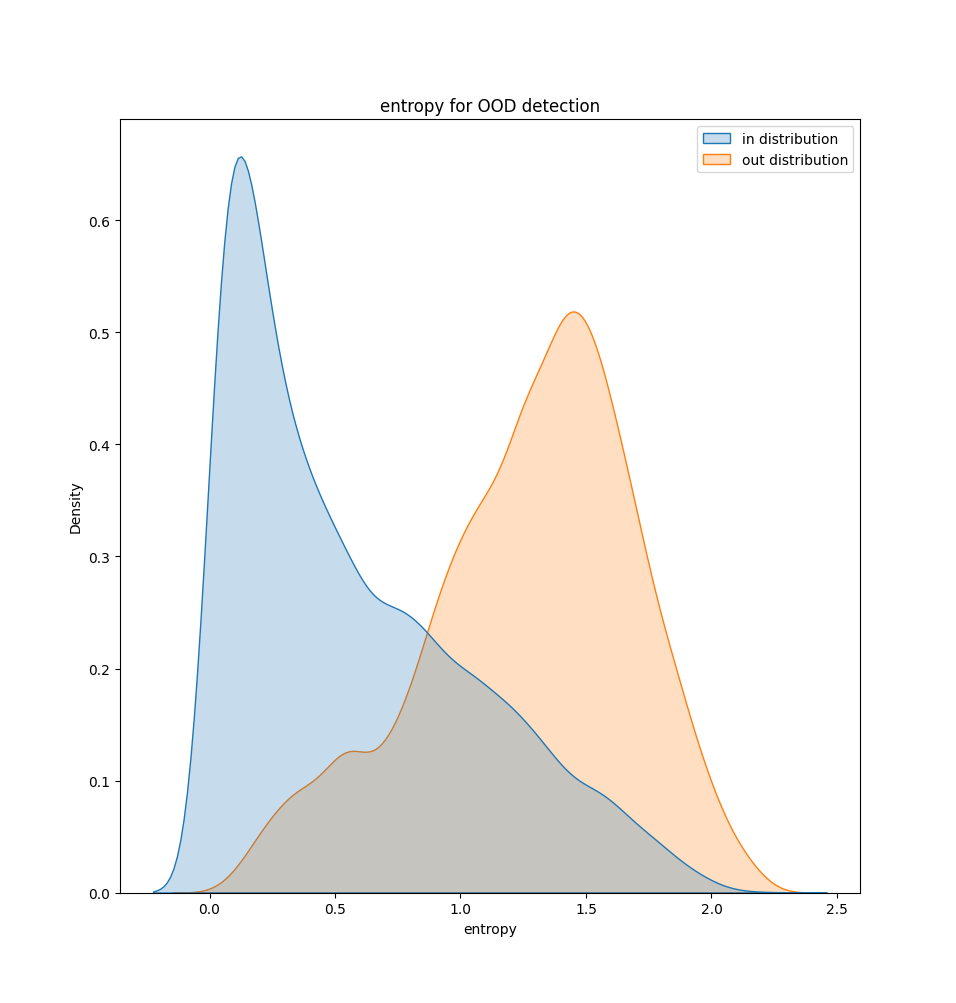
\includegraphics[width=.9\linewidth]{./ens_mnist_entropy.png}
\caption{\label{fig:org62b3204}
Ensemble (ID mnist) Entropy}
\end{figure}

\begin{figure}[htbp]
\centering
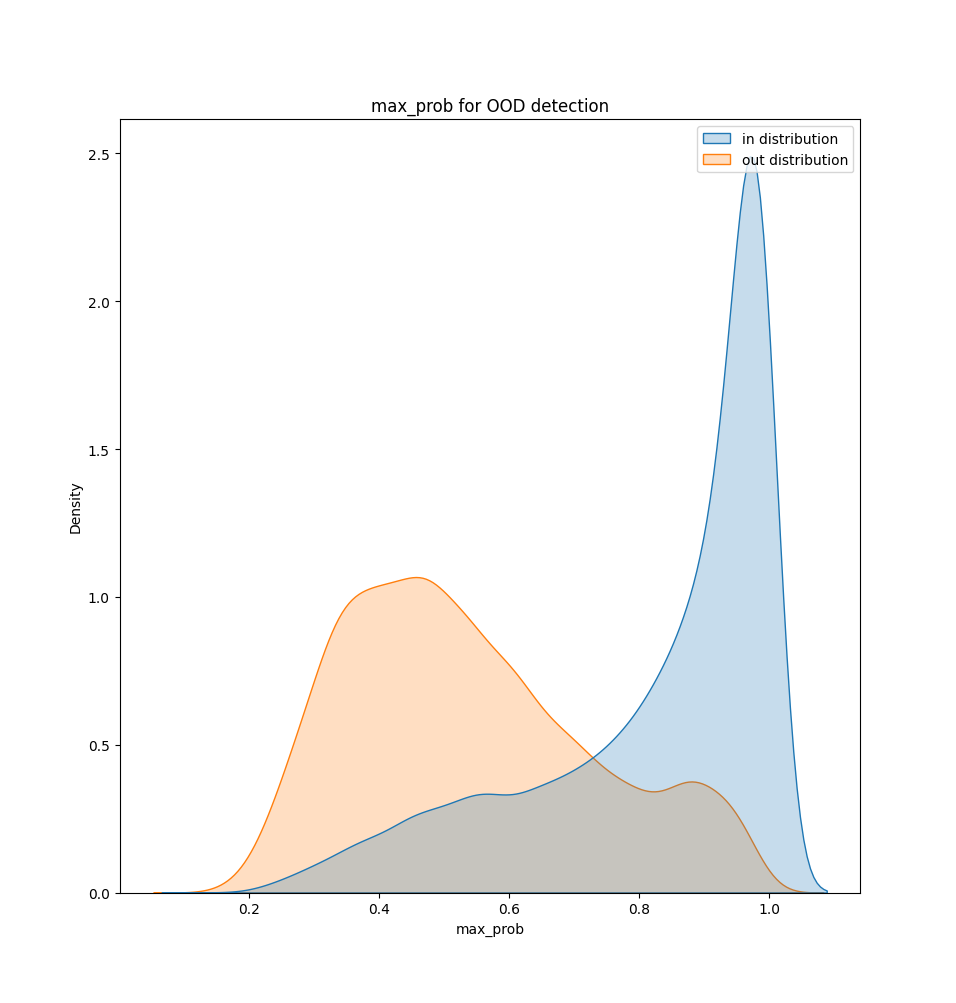
\includegraphics[width=.9\linewidth]{./ens_mnist_max_prob.png}
\caption{\label{fig:org270c432}
Ensemble (ID mnist) Max Probabilities}
\end{figure}

\begin{figure}[htbp]
\centering
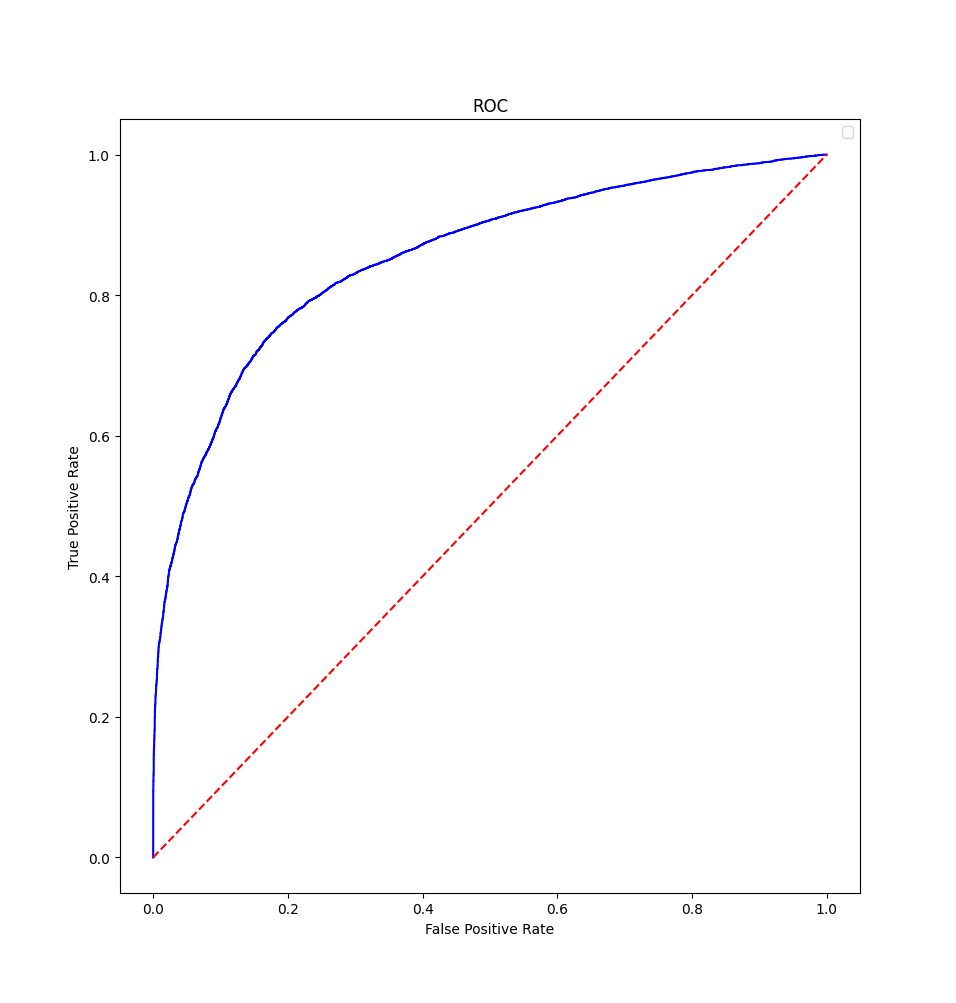
\includegraphics[width=.9\linewidth]{./ens_mnist_roc.png}
\caption{\label{fig:org9599962}
Ensemble (ID mnist) ROC curve}
\end{figure}

\begin{figure}[htbp]
\centering
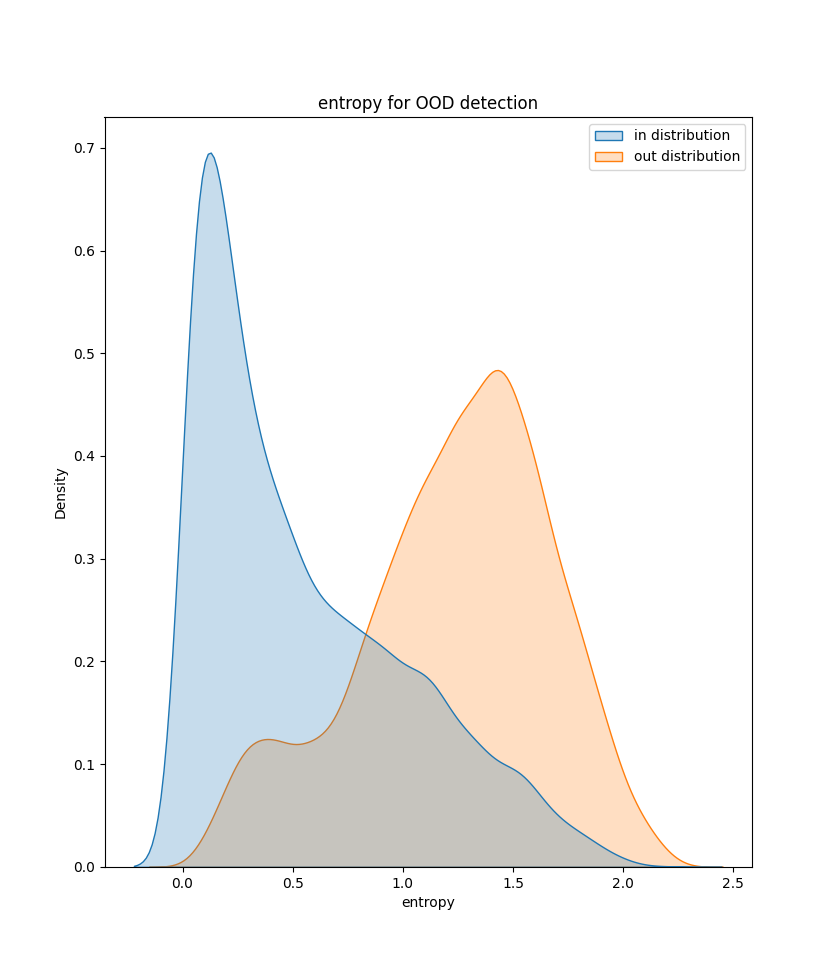
\includegraphics[width=.9\linewidth]{./base_mnist_entropy.png}
\caption{\label{fig:orgdeb9a27}
Baseline (ID mnist) Entropy}
\end{figure}

\begin{figure}[htbp]
\centering
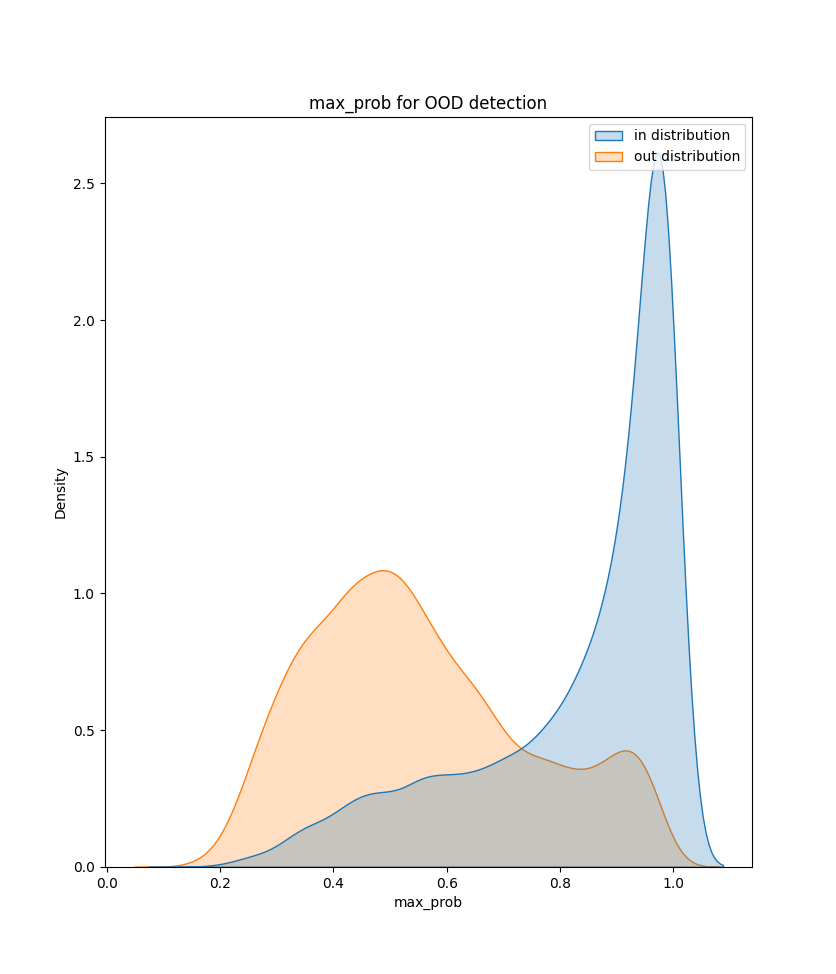
\includegraphics[width=.9\linewidth]{./base_mnist_max_prob.png}
\caption{\label{fig:org9621000}
Baseline (ID mnist) Max Probabilities}
\end{figure}

\begin{figure}[htbp]
\centering
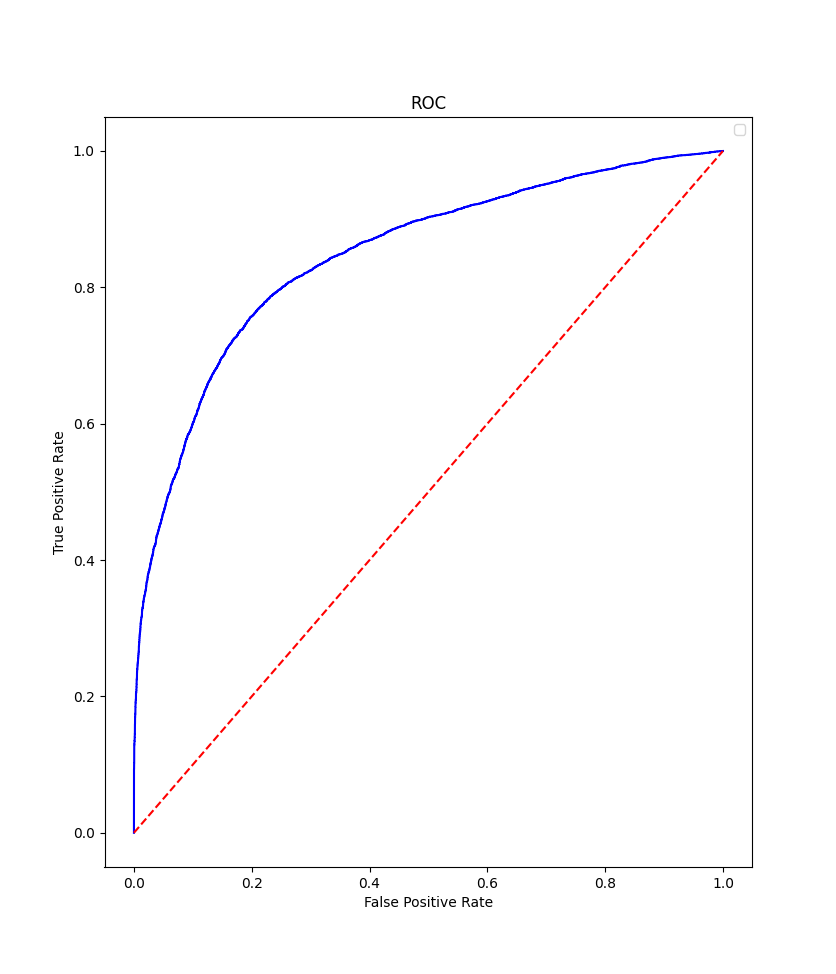
\includegraphics[width=.9\linewidth]{./base_mnist_roc.png}
\caption{\label{fig:org3cd6800}
Baseline (ID mnist) ROC curve}
\end{figure}

\begin{figure}[htbp]
\centering
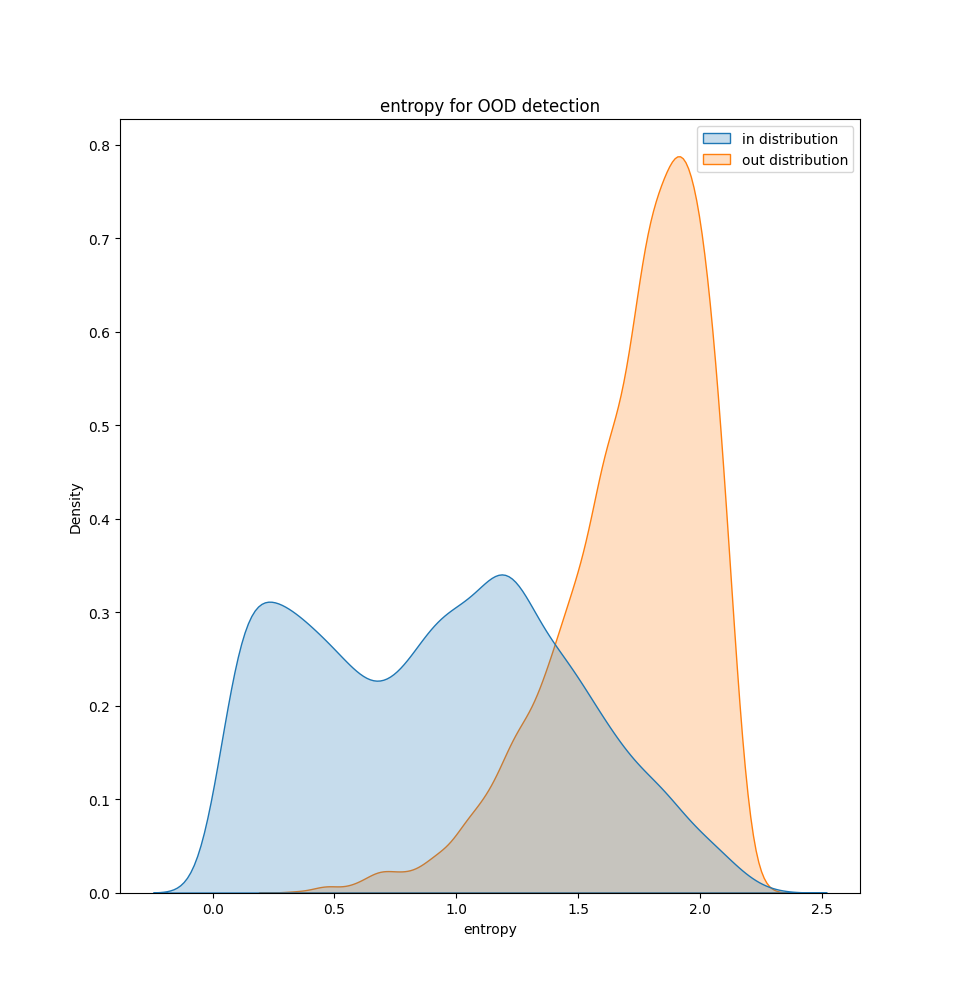
\includegraphics[width=.9\linewidth]{./ens_fash_entropy.png}
\caption{\label{fig:org38b1854}
Ensemble (ID fashion\(_{\text{mnist}}\)) Entropy}
\end{figure}

\begin{figure}[htbp]
\centering
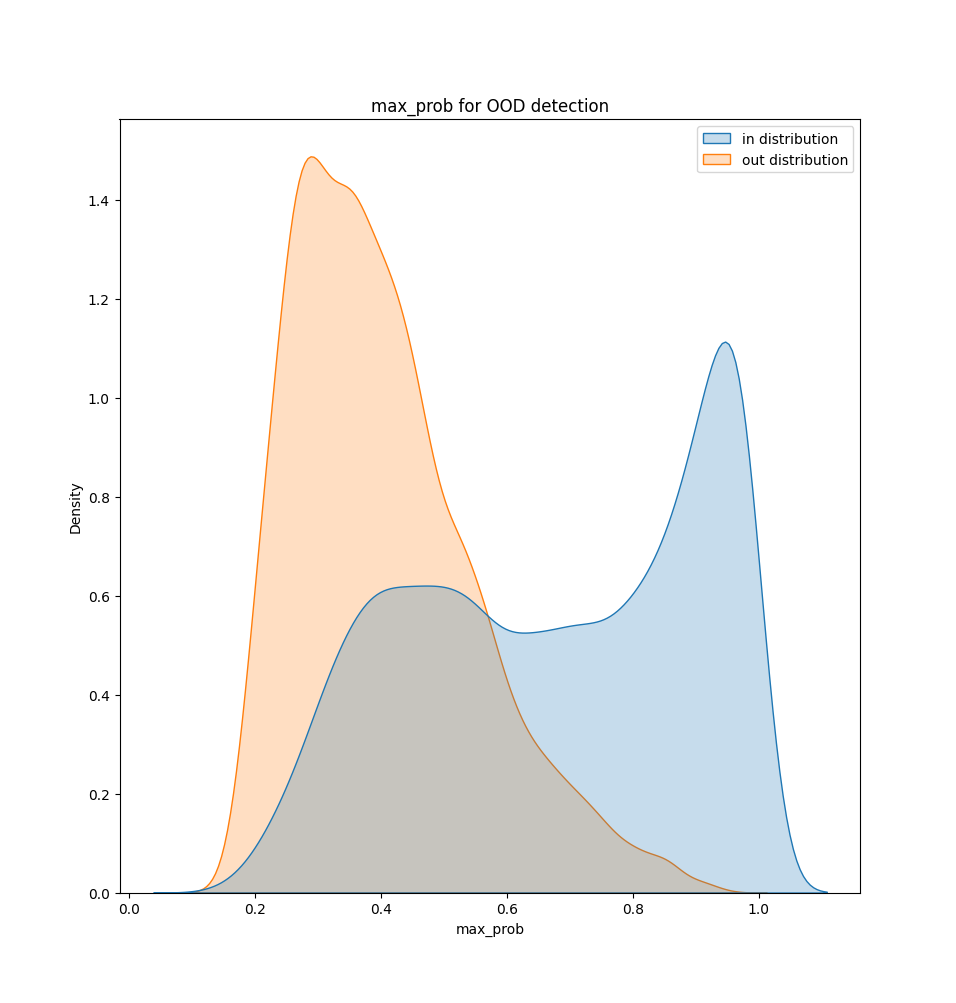
\includegraphics[width=.9\linewidth]{./ens_fash_max_prob.png}
\caption{\label{fig:orgb9eb82d}
Ensemble (ID fashion\(_{\text{mnist}}\)) Max Probabilities}
\end{figure}

\begin{figure}[htbp]
\centering
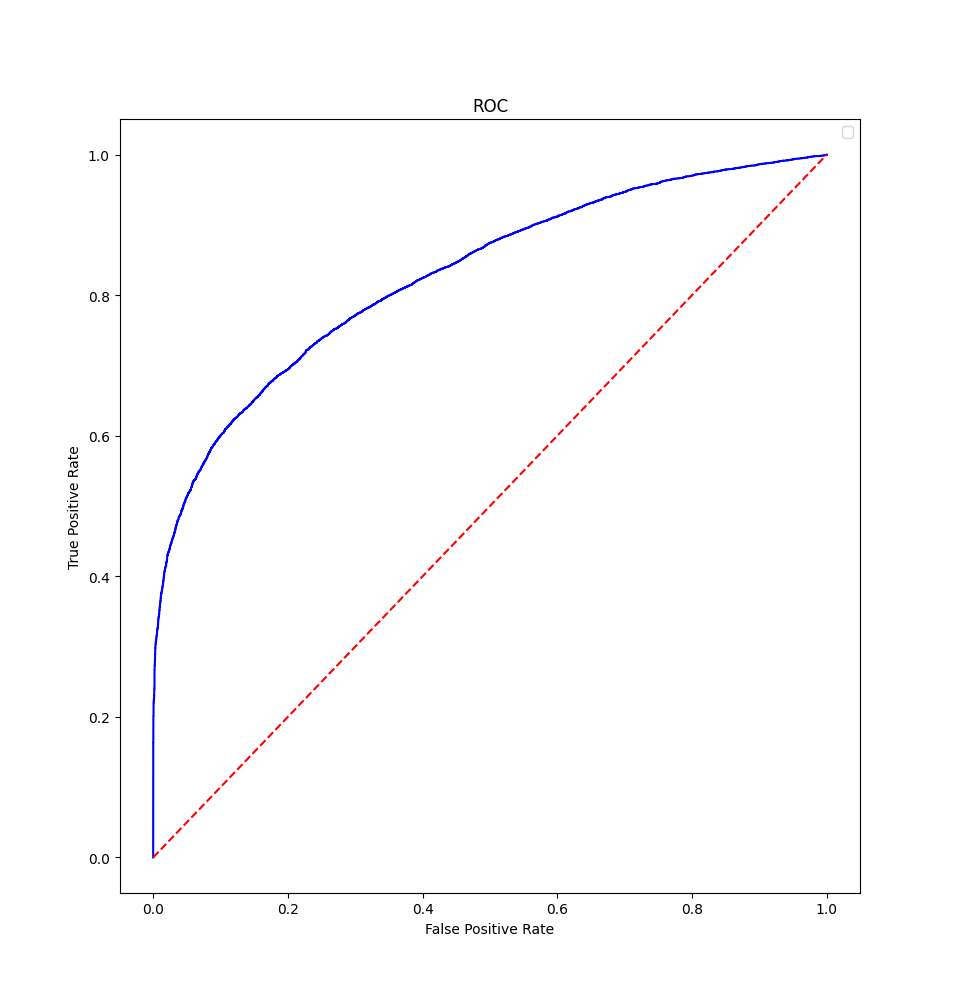
\includegraphics[width=.9\linewidth]{./ens_fash_roc.png}
\caption{\label{fig:org279ec8c}
Ensemble (ID fashion\(_{\text{mnist}}\)) ROC curve}
\end{figure}

\begin{figure}[htbp]
\centering
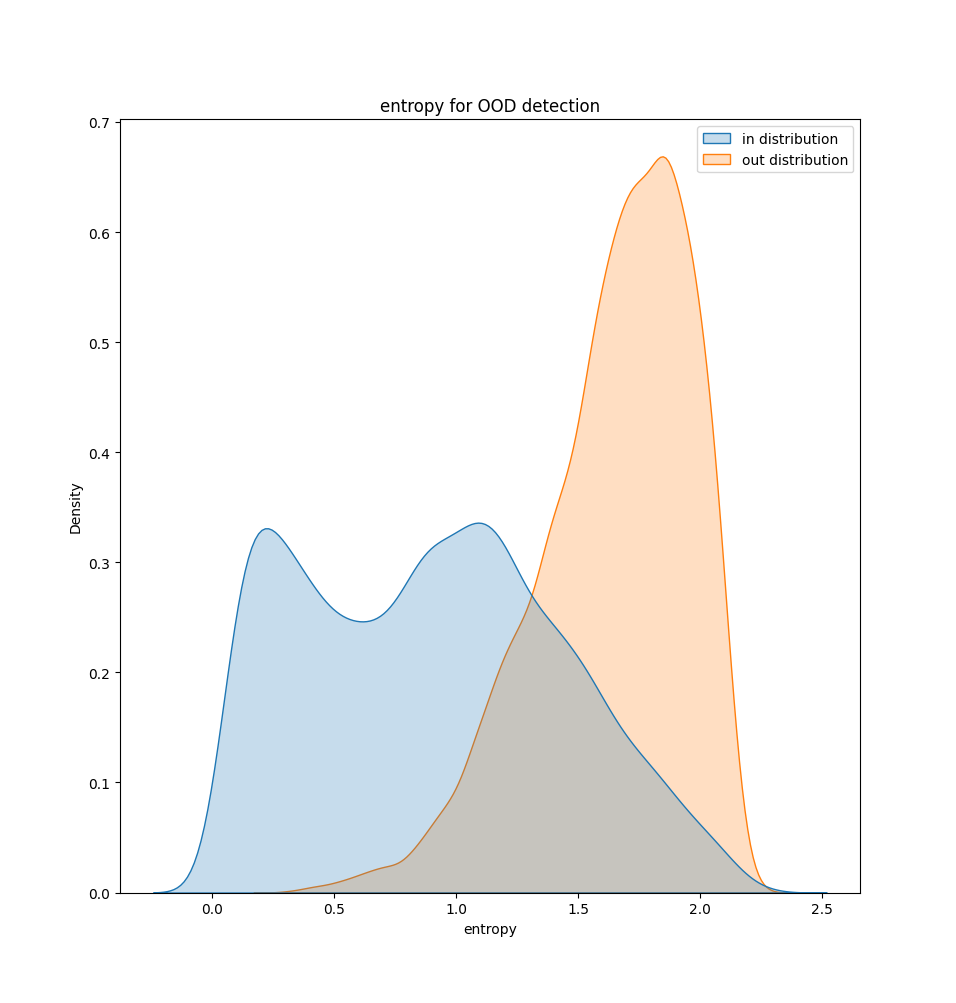
\includegraphics[width=.9\linewidth]{./base_fash_entropy.png}
\caption{\label{fig:org48f3c2d}
Baseline (ID fashion\(_{\text{mnist}}\)) Entropy}
\end{figure}

\begin{figure}[htbp]
\centering
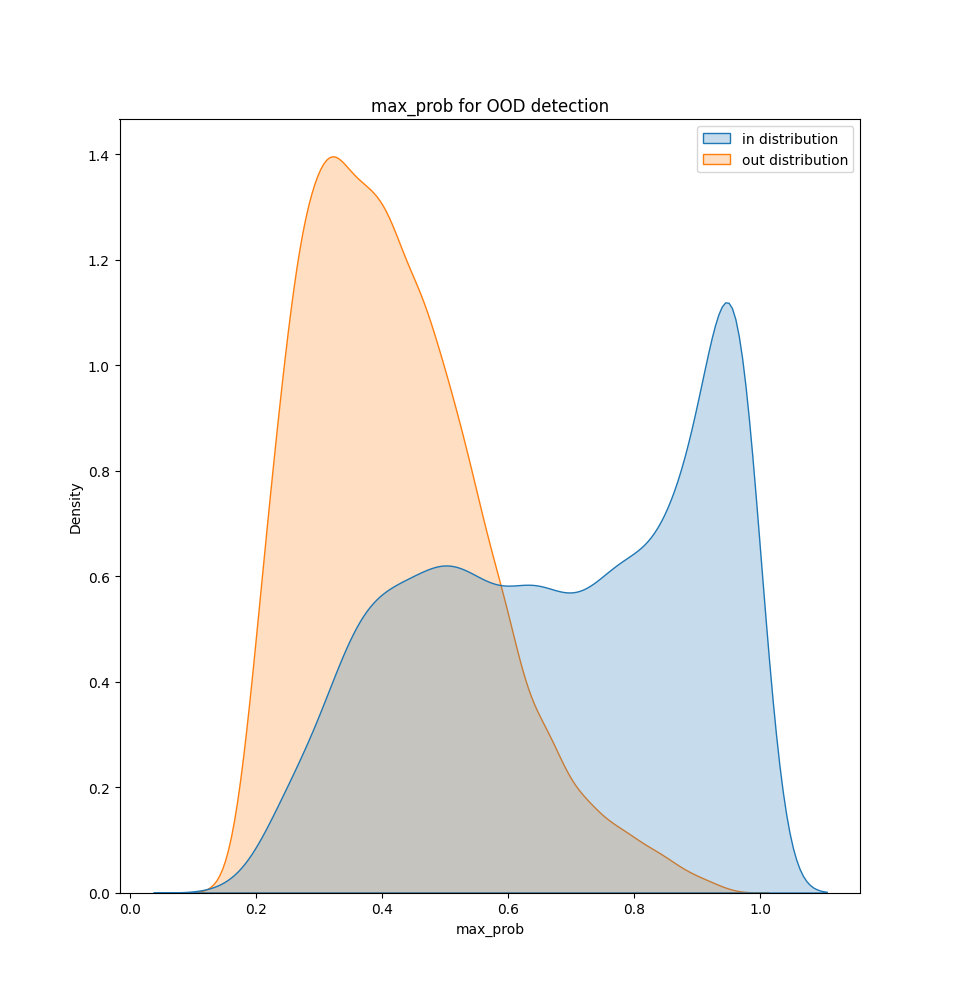
\includegraphics[width=.9\linewidth]{./base_fash_max_prob.png}
\caption{\label{fig:org90b94ba}
Baseline (ID fashion\(_{\text{mnist}}\)) Max Probabilities}
\end{figure}

\begin{figure}[htbp]
\centering
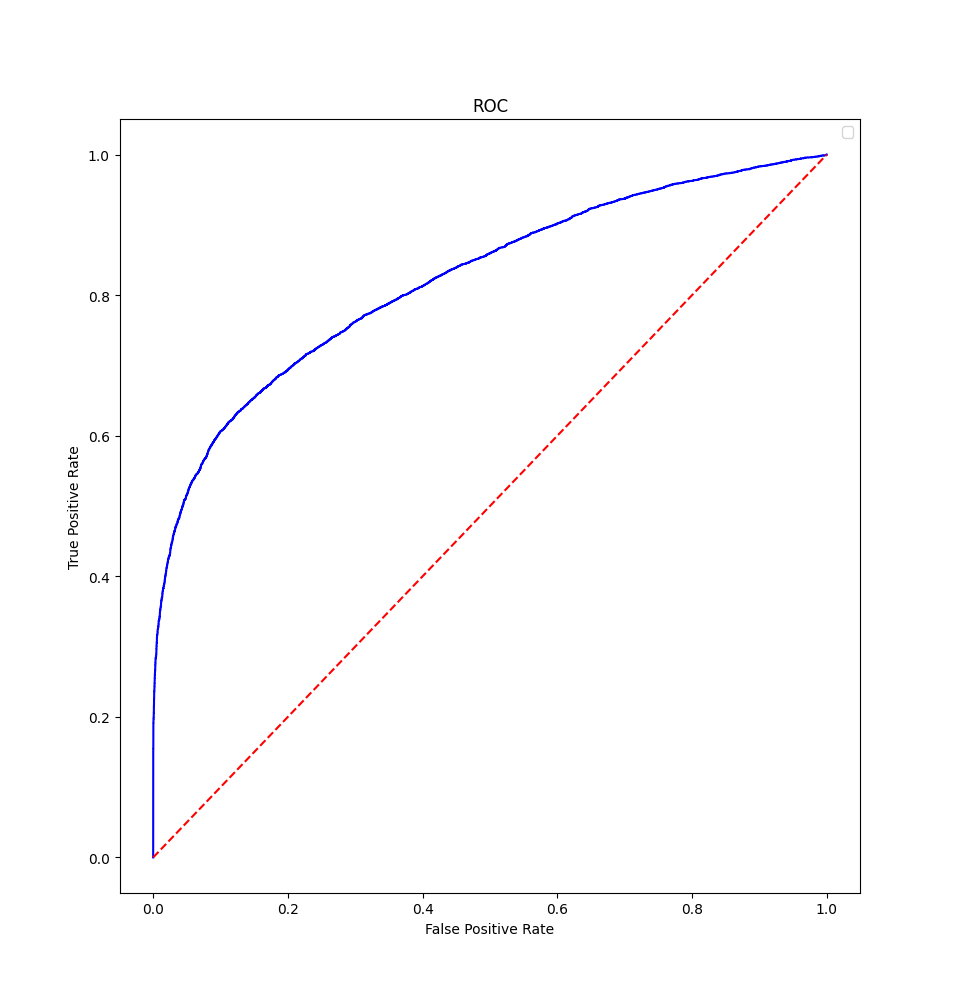
\includegraphics[width=.9\linewidth]{./base_fash_roc.png}
\caption{\label{fig:org42337be}
Baseline (ID fashion\(_{\text{mnist}}\)) ROC curve}
\end{figure}



\begin{figure}[htbp]
\centering
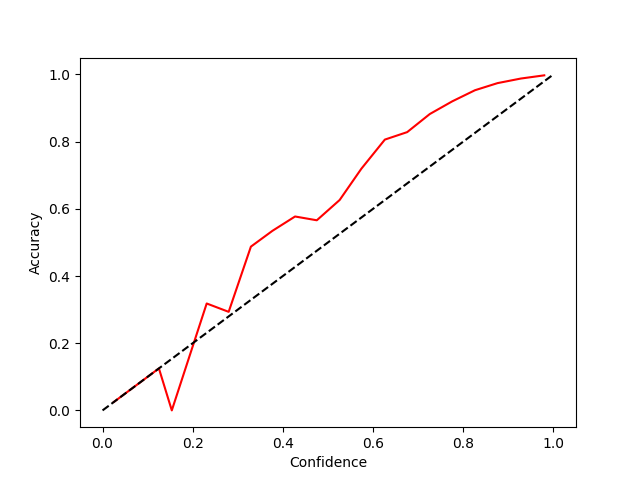
\includegraphics[width=.9\linewidth]{./ens_mnist_total_rel.png}
\caption{\label{fig:orgf37ac26}
Ensemble Reliability Plot (ID mnist)}
\end{figure}

\begin{figure}[htbp]
\centering
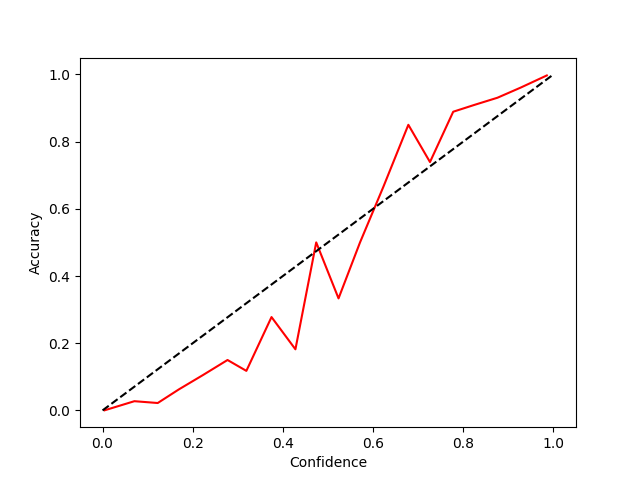
\includegraphics[width=.9\linewidth]{./ens_mnist_rel_0.png}
\caption{\label{fig:org304bcac}
Ensemble Reliability Plot for class 0 (ID mnist)}
\end{figure}

\begin{figure}[htbp]
\centering
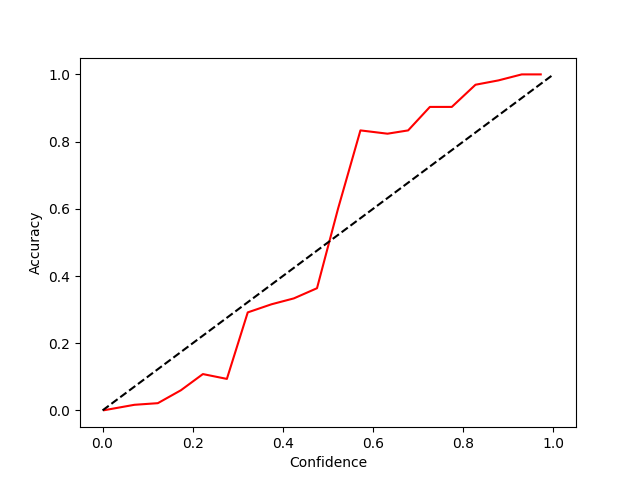
\includegraphics[width=.9\linewidth]{./ens_mnist_rel_1.png}
\caption{\label{fig:org371cd14}
Ensemble Reliability Plot for class 1 (ID mnist)}
\end{figure}

\begin{figure}[htbp]
\centering
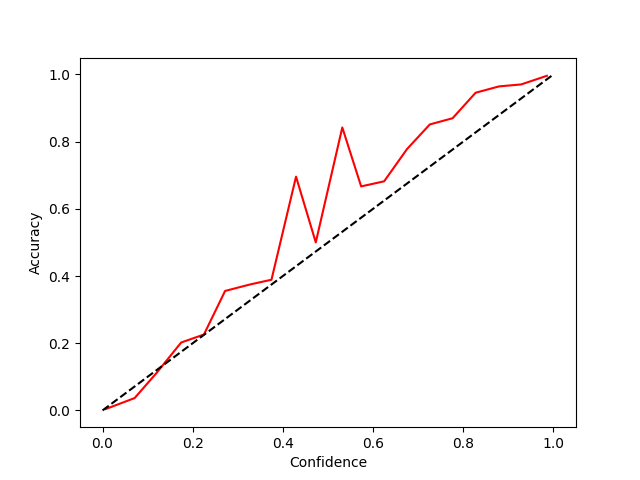
\includegraphics[width=.9\linewidth]{./ens_mnist_rel_2.png}
\caption{\label{fig:orga775273}
Ensemble Reliability Plot for class 2 (ID mnist)}
\end{figure}

\begin{figure}[htbp]
\centering
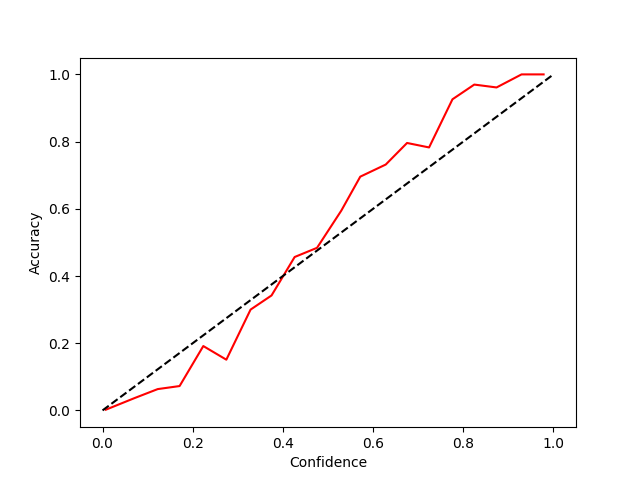
\includegraphics[width=.9\linewidth]{./ens_mnist_rel_3.png}
\caption{\label{fig:org7248ef0}
Ensemble Reliability Plot for class 3 (ID mnist)}
\end{figure}

\begin{figure}[htbp]
\centering
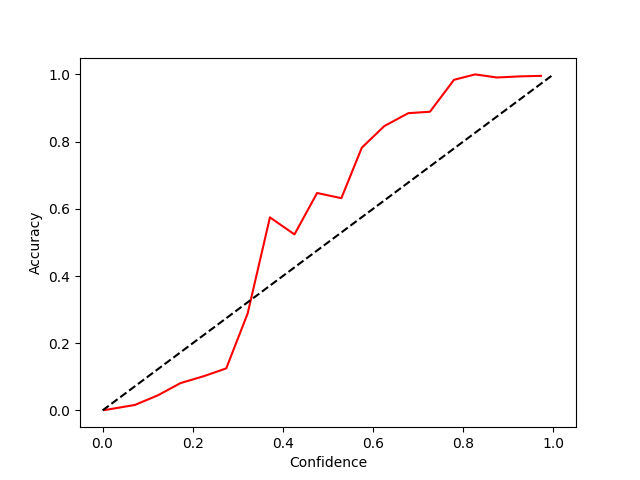
\includegraphics[width=.9\linewidth]{./ens_mnist_rel_4.png}
\caption{\label{fig:org14e7042}
Ensemble Reliability Plot for class 4 (ID mnist)}
\end{figure}

\begin{figure}[htbp]
\centering
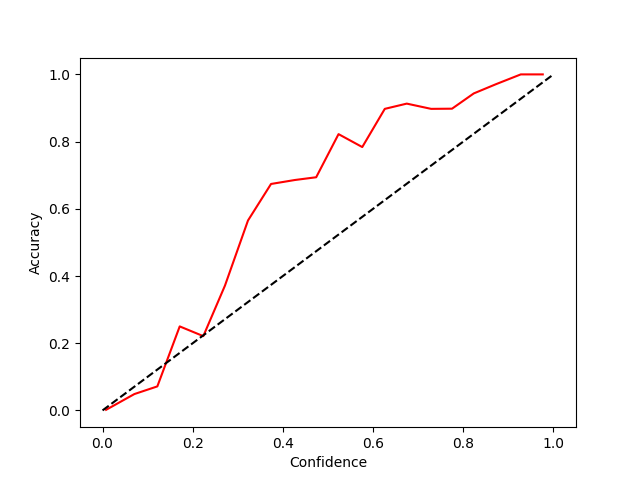
\includegraphics[width=.9\linewidth]{./ens_mnist_rel_5.png}
\caption{\label{fig:orgfde6cc2}
Ensemble Reliability Plot for class 5 (ID mnist)}
\end{figure}

\begin{figure}[htbp]
\centering
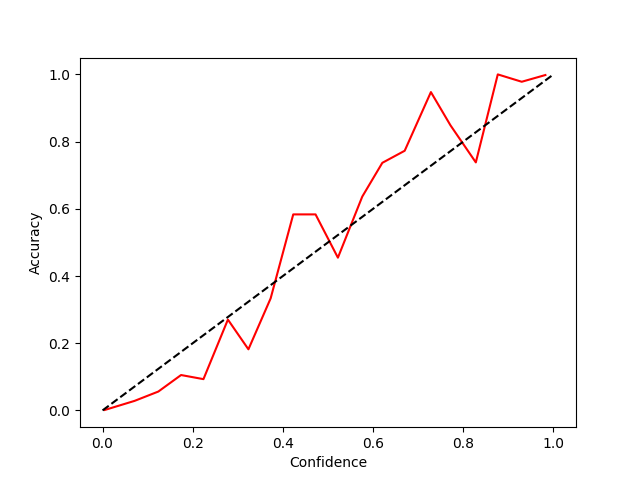
\includegraphics[width=.9\linewidth]{./ens_mnist_rel_6.png}
\caption{\label{fig:orgcacddd3}
Ensemble Reliability Plot for class 6 (ID mnist)}
\end{figure}

\begin{figure}[htbp]
\centering
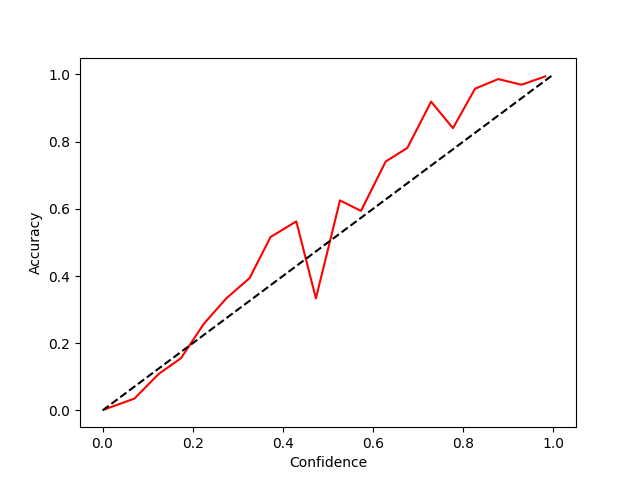
\includegraphics[width=.9\linewidth]{./ens_mnist_rel_7.png}
\caption{\label{fig:org9fdb3b5}
Ensemble Reliability Plot for class 7 (ID mnist)}
\end{figure}

\begin{figure}[htbp]
\centering
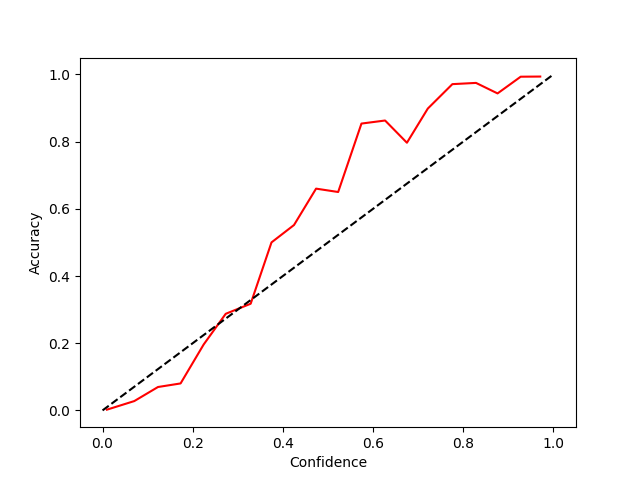
\includegraphics[width=.9\linewidth]{./ens_mnist_rel_8.png}
\caption{\label{fig:org716d9d3}
Ensemble Reliability Plot for class 8 (ID mnist)}
\end{figure}

\begin{figure}[htbp]
\centering
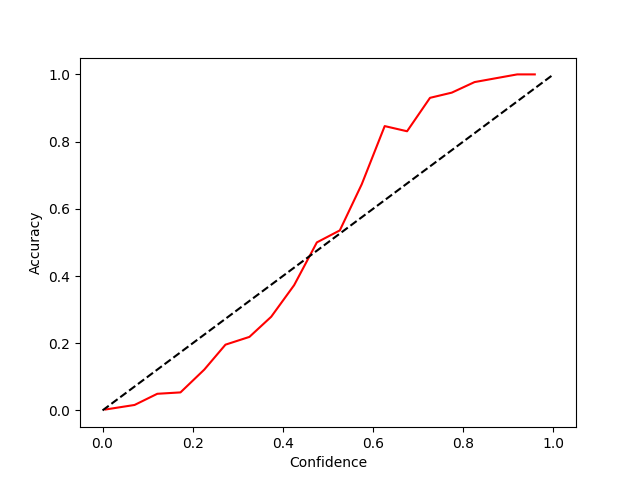
\includegraphics[width=.9\linewidth]{./ens_mnist_rel_9.png}
\caption{\label{fig:org1229dcd}
Ensemble Reliability Plot for class 9 (ID mnist)}
\end{figure}

\begin{figure}[htbp]
\centering
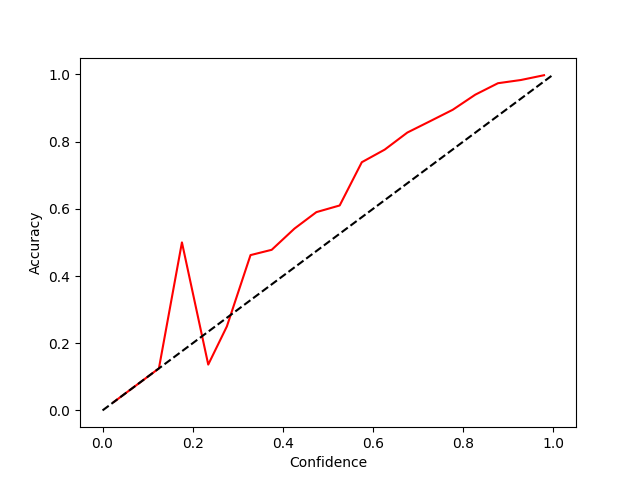
\includegraphics[width=.9\linewidth]{./base_mnist_total_rel.png}
\caption{\label{fig:orgcf4aed6}
Baseline Reliability Plot (ID mnist)}
\end{figure}

\begin{figure}[htbp]
\centering
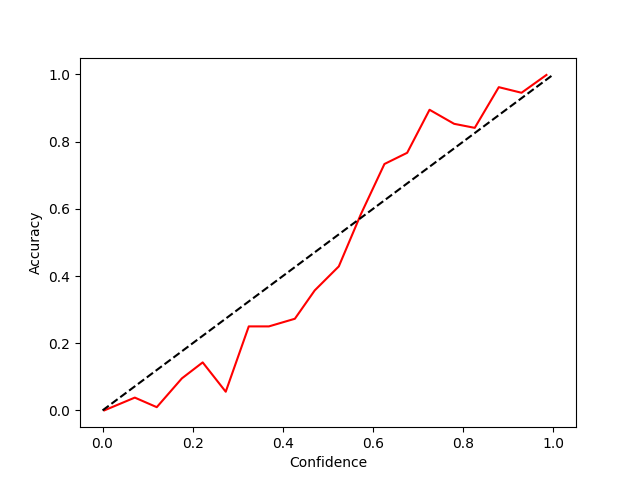
\includegraphics[width=.9\linewidth]{./base_mnist_rel_0.png}
\caption{\label{fig:org48426c1}
Baseline Reliability Plot for class 0 (ID mnist)}
\end{figure}

\begin{figure}[htbp]
\centering
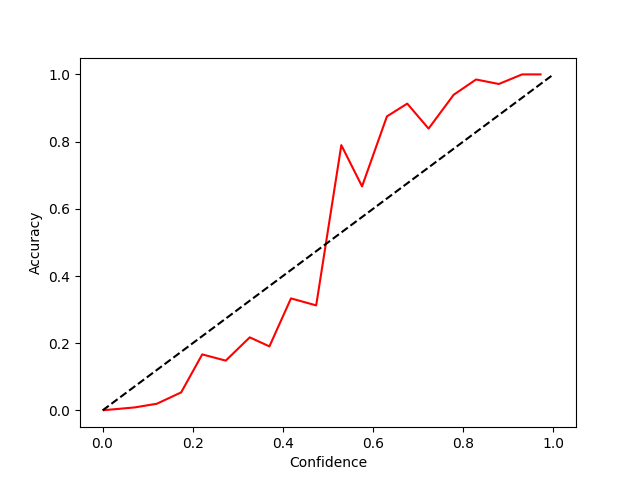
\includegraphics[width=.9\linewidth]{./base_mnist_rel_1.png}
\caption{\label{fig:orgf25634d}
Baseline Reliability Plot for class 1 (ID mnist)}
\end{figure}

\begin{figure}[htbp]
\centering
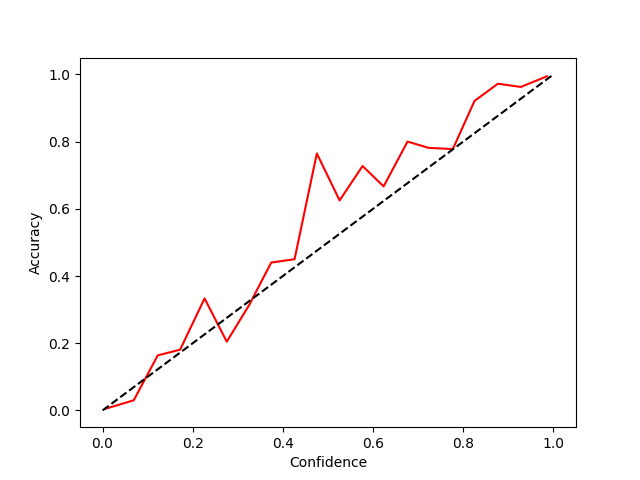
\includegraphics[width=.9\linewidth]{./base_mnist_rel_2.png}
\caption{\label{fig:org03feedd}
Baseline Reliability Plot for class 2 (ID mnist)}
\end{figure}

\begin{figure}[htbp]
\centering
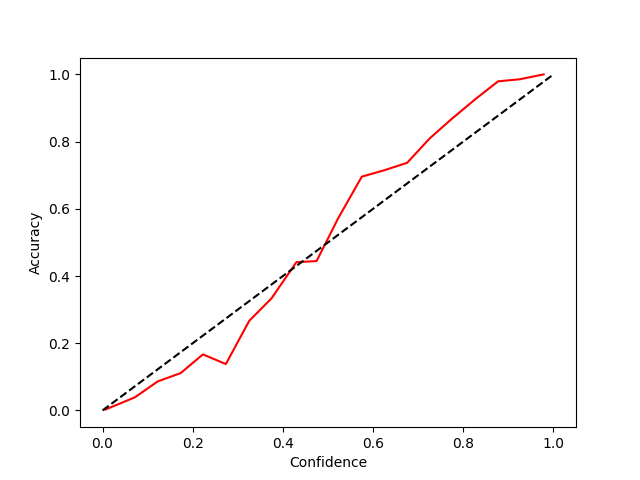
\includegraphics[width=.9\linewidth]{./base_mnist_rel_3.png}
\caption{\label{fig:orgeebf6df}
Baseline Reliability Plot for class 3 (ID mnist)}
\end{figure}

\begin{figure}[htbp]
\centering
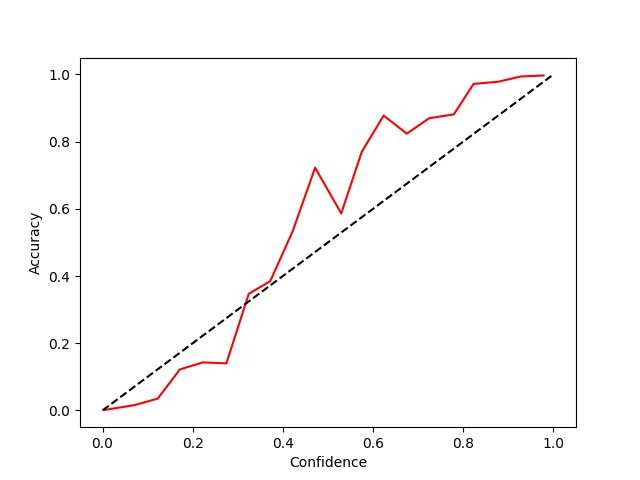
\includegraphics[width=.9\linewidth]{./base_mnist_rel_4.png}
\caption{\label{fig:org7816d2a}
Baseline Reliability Plot for class 4 (ID mnist)}
\end{figure}

\begin{figure}[htbp]
\centering
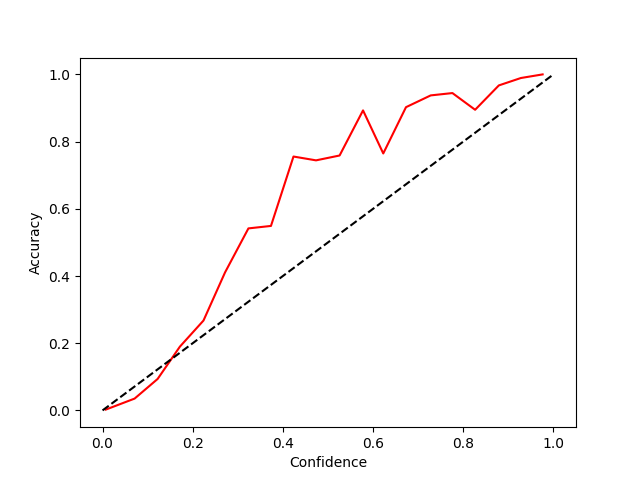
\includegraphics[width=.9\linewidth]{./base_mnist_rel_5.png}
\caption{\label{fig:org9f9deca}
Baseline Reliability Plot for class 5 (ID mnist)}
\end{figure}

\begin{figure}[htbp]
\centering
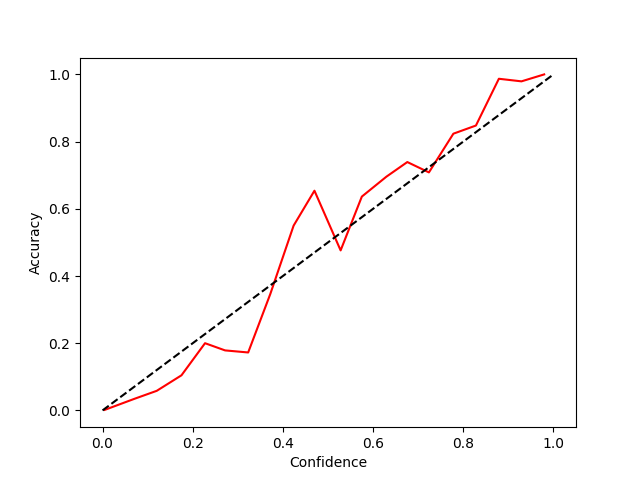
\includegraphics[width=.9\linewidth]{./base_mnist_rel_6.png}
\caption{\label{fig:org260d8e7}
Baseline Reliability Plot for class 6 (ID mnist)}
\end{figure}

\begin{figure}[htbp]
\centering
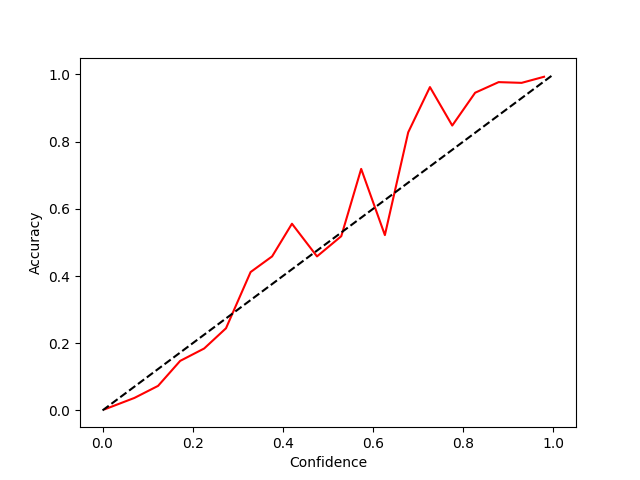
\includegraphics[width=.9\linewidth]{./base_mnist_rel_7.png}
\caption{\label{fig:orgc5350fc}
Baseline Reliability Plot for class 7 (ID mnist)}
\end{figure}

\begin{figure}[htbp]
\centering
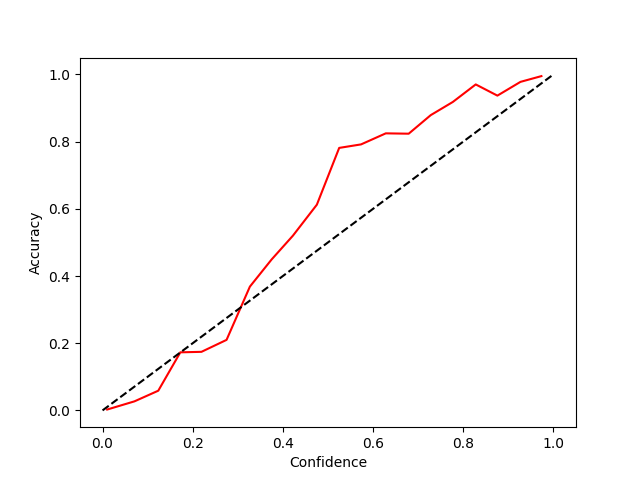
\includegraphics[width=.9\linewidth]{./base_mnist_rel_8.png}
\caption{\label{fig:orgaaaec75}
Baseline Reliability Plot for class 8 (ID mnist)}
\end{figure}

\begin{figure}[htbp]
\centering
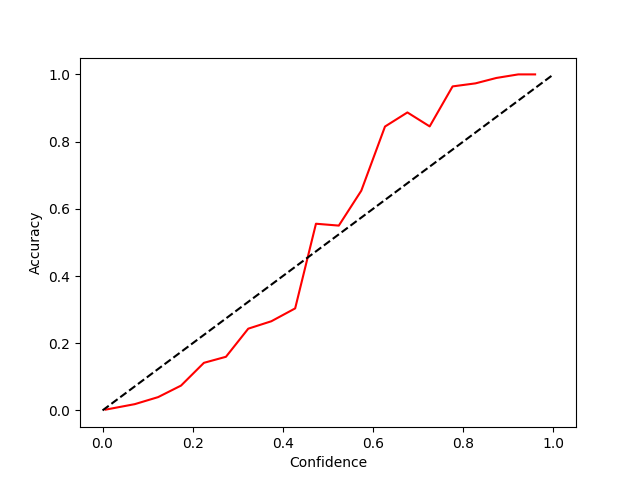
\includegraphics[width=.9\linewidth]{./base_mnist_rel_9.png}
\caption{\label{fig:org50c142f}
Baseline Reliability Plot for class 9 (ID mnist)}
\end{figure}

\begin{figure}[htbp]
\centering
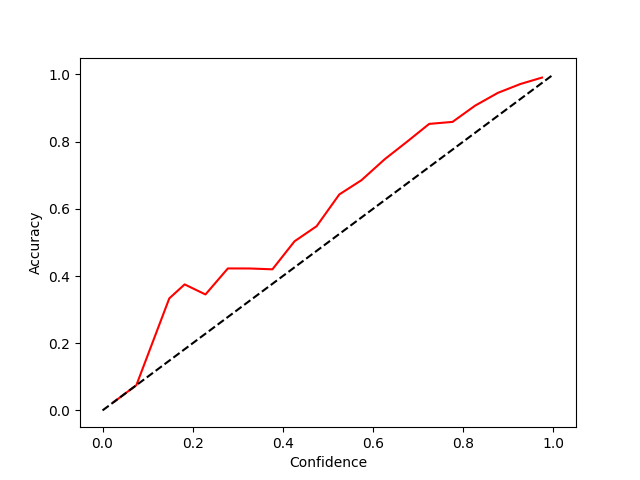
\includegraphics[width=.9\linewidth]{./ens_fash_total_rel.png}
\caption{\label{fig:orga2055a7}
Ensemble Reliability Plot (ID fash)}
\end{figure}

\begin{figure}[htbp]
\centering
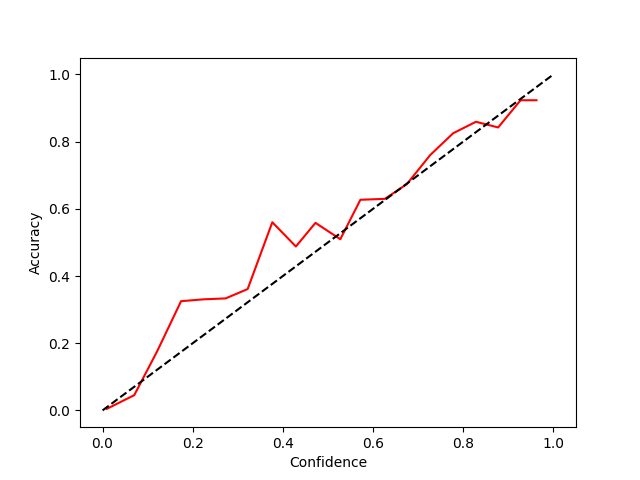
\includegraphics[width=.9\linewidth]{./ens_fash_rel_0.png}
\caption{\label{fig:org9f5f3da}
Ensemble Reliability Plot for class 0 (ID fash)}
\end{figure}

\begin{figure}[htbp]
\centering
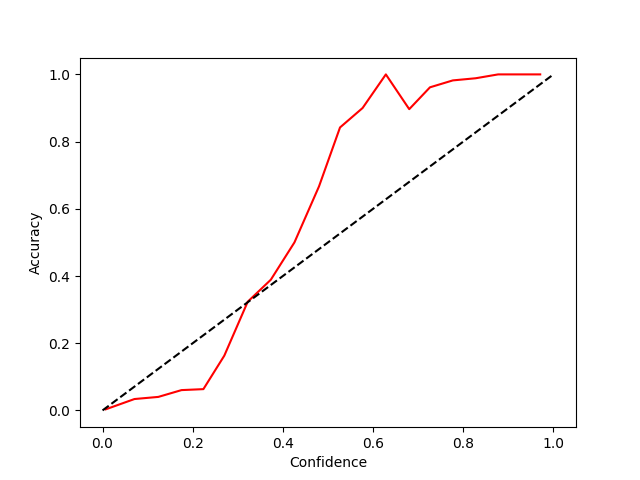
\includegraphics[width=.9\linewidth]{./ens_fash_rel_1.png}
\caption{\label{fig:orgca3bd5f}
Ensemble Reliability Plot for class 1 (ID fash)}
\end{figure}

\begin{figure}[htbp]
\centering
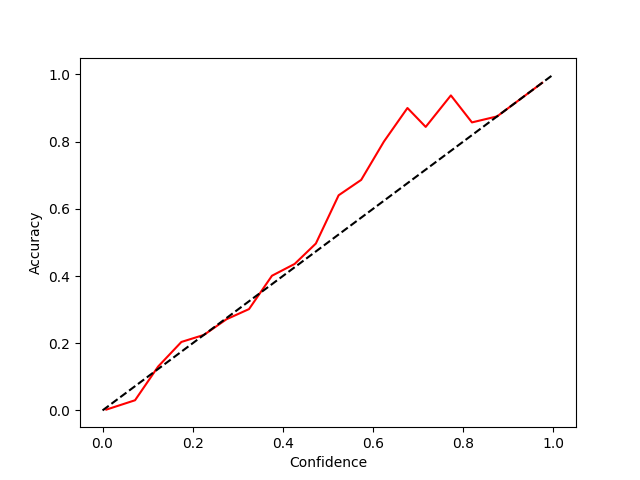
\includegraphics[width=.9\linewidth]{./ens_fash_rel_2.png}
\caption{\label{fig:org4c4dbb2}
Ensemble Reliability Plot for class 2 (ID fash)}
\end{figure}

\begin{figure}[htbp]
\centering
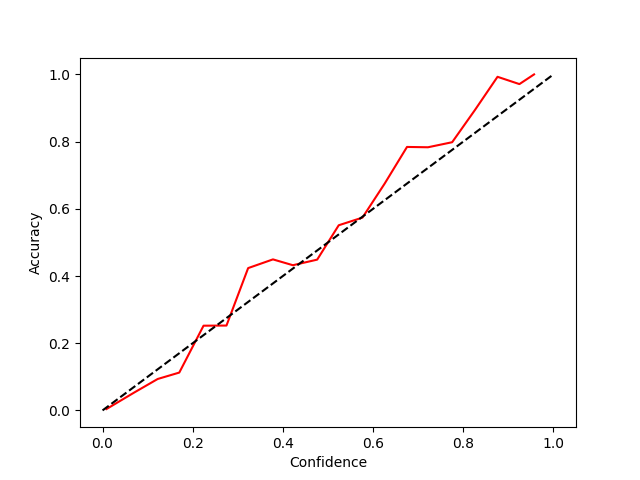
\includegraphics[width=.9\linewidth]{./ens_fash_rel_3.png}
\caption{\label{fig:org5777caa}
Ensemble Reliability Plot for class 3 (ID fash)}
\end{figure}

\begin{figure}[htbp]
\centering
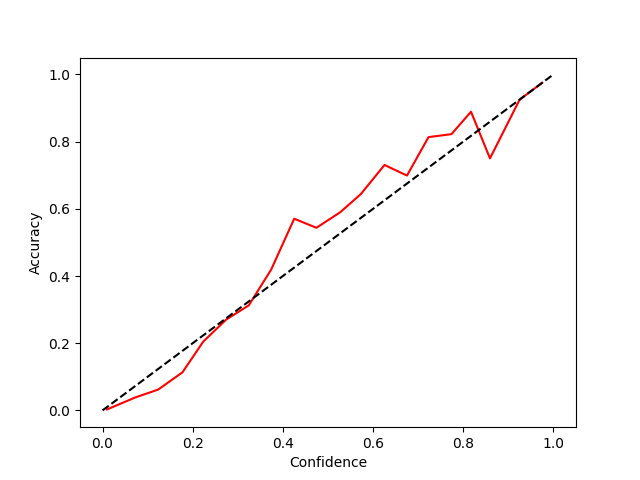
\includegraphics[width=.9\linewidth]{./ens_fash_rel_4.png}
\caption{\label{fig:org11503c5}
Ensemble Reliability Plot for class 4 (ID fash)}
\end{figure}

\begin{figure}[htbp]
\centering
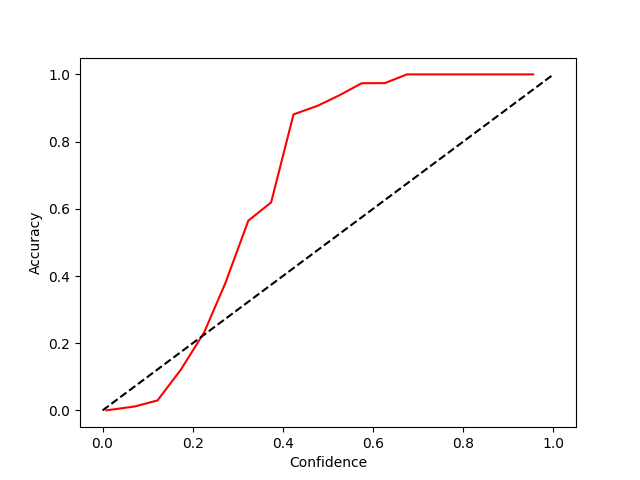
\includegraphics[width=.9\linewidth]{./ens_fash_rel_5.png}
\caption{\label{fig:orgaf3af93}
Ensemble Reliability Plot for class 5 (ID fash)}
\end{figure}

\begin{figure}[htbp]
\centering
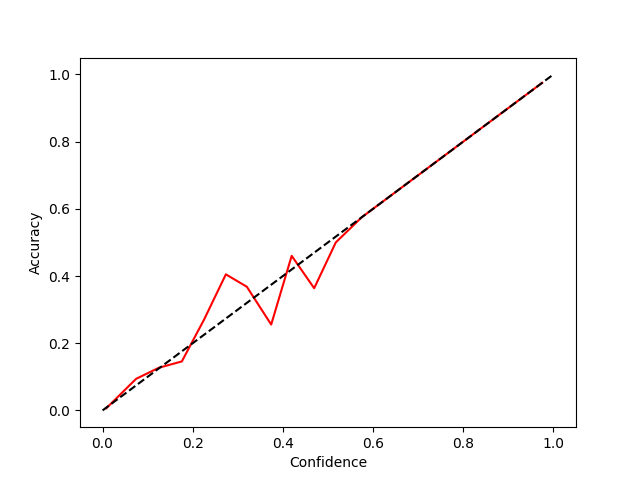
\includegraphics[width=.9\linewidth]{./ens_fash_rel_6.png}
\caption{\label{fig:org5fd780b}
Ensemble Reliability Plot for class 6 (ID fash)}
\end{figure}

\begin{figure}[htbp]
\centering
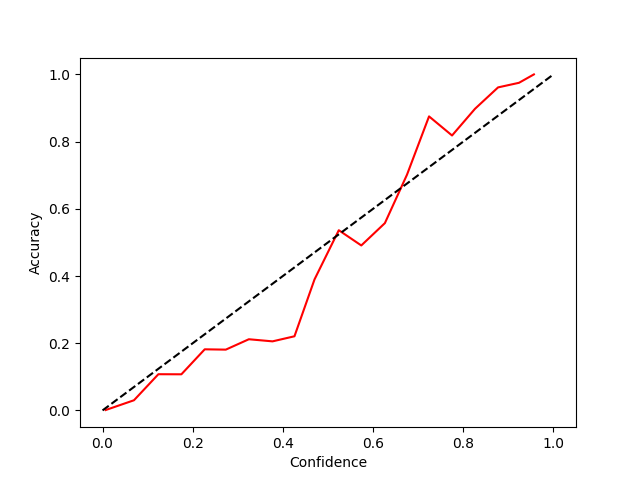
\includegraphics[width=.9\linewidth]{./ens_fash_rel_7.png}
\caption{\label{fig:orgadca54a}
Ensemble Reliability Plot for class 7 (ID fash)}
\end{figure}

\begin{figure}[htbp]
\centering
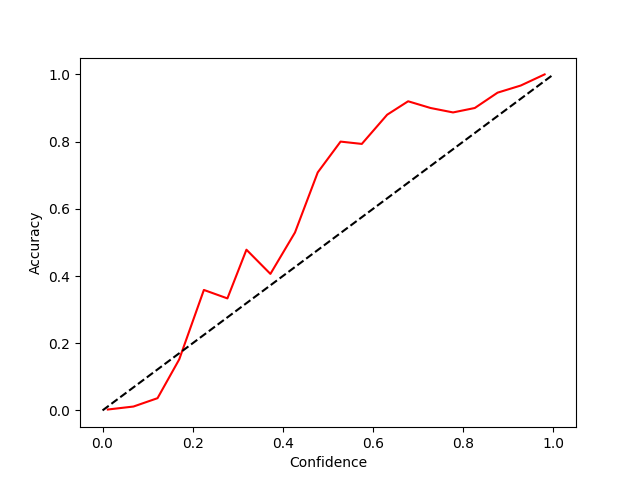
\includegraphics[width=.9\linewidth]{./ens_fash_rel_8.png}
\caption{\label{fig:org01f3666}
Ensemble Reliability Plot for class 8 (ID fash)}
\end{figure}

\begin{figure}[htbp]
\centering
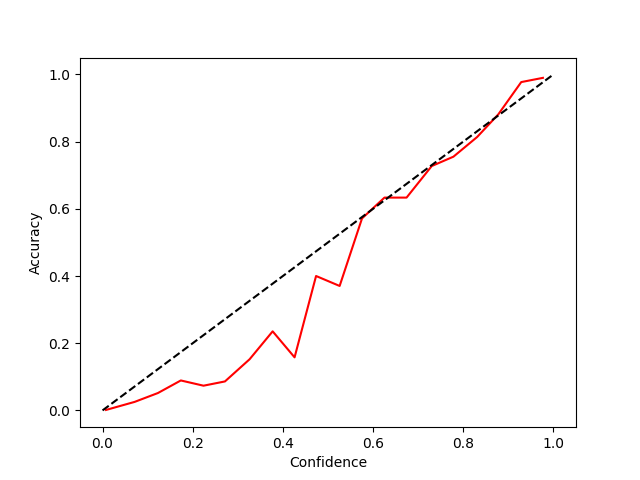
\includegraphics[width=.9\linewidth]{./ens_fash_rel_9.png}
\caption{\label{fig:orgdc938ca}
Ensemble Reliability Plot for class 9 (ID fash)}
\end{figure}
\end{document}
